% Created 2021-09-27 Mon 12:02
% Intended LaTeX compiler: xelatex
\documentclass[letterpaper]{article}
\usepackage{graphicx}
\usepackage{grffile}
\usepackage{longtable}
\usepackage{wrapfig}
\usepackage{rotating}
\usepackage[normalem]{ulem}
\usepackage{amsmath}
\usepackage{textcomp}
\usepackage{amssymb}
\usepackage{capt-of}
\usepackage{hyperref}
\setlength{\parindent}{0pt}
\usepackage[margin=1in]{geometry}
\usepackage{fontspec}
\usepackage{svg}
\usepackage{cancel}
\usepackage{indentfirst}
\setmainfont[ItalicFont = LiberationSans-Italic, BoldFont = LiberationSans-Bold, BoldItalicFont = LiberationSans-BoldItalic]{LiberationSans}
\newfontfamily\NHLight[ItalicFont = LiberationSansNarrow-Italic, BoldFont       = LiberationSansNarrow-Bold, BoldItalicFont = LiberationSansNarrow-BoldItalic]{LiberationSansNarrow}
\newcommand\textrmlf[1]{{\NHLight#1}}
\newcommand\textitlf[1]{{\NHLight\itshape#1}}
\let\textbflf\textrm
\newcommand\textulf[1]{{\NHLight\bfseries#1}}
\newcommand\textuitlf[1]{{\NHLight\bfseries\itshape#1}}
\usepackage{fancyhdr}
\pagestyle{fancy}
\usepackage{titlesec}
\usepackage{titling}
\makeatletter
\lhead{\textbf{\@title}}
\makeatother
\rhead{\textrmlf{Compiled} \today}
\lfoot{\theauthor\ \textbullet \ \textbf{2021-2022}}
\cfoot{}
\rfoot{\textrmlf{Page} \thepage}
\renewcommand{\tableofcontents}{}
\titleformat{\section} {\Large} {\textrmlf{\thesection} {|}} {0.3em} {\textbf}
\titleformat{\subsection} {\large} {\textrmlf{\thesubsection} {|}} {0.2em} {\textbf}
\titleformat{\subsubsection} {\large} {\textrmlf{\thesubsubsection} {|}} {0.1em} {\textbf}
\setlength{\parskip}{0.45em}
\renewcommand\maketitle{}
\author{Houjun Liu}
\date{\today}
\title{Voltage}
\hypersetup{
 pdfauthor={Houjun Liu},
 pdftitle={Voltage},
 pdfkeywords={},
 pdfsubject={},
 pdfcreator={Emacs 28.0.50 (Org mode 9.4.4)}, 
 pdflang={English}}
\begin{document}

\tableofcontents



\section{Voltage}
\label{sec:org7ee28fd}
\subsection{First, a geography thing.}
\label{sec:org9e5d837}
\begin{figure}[htbp]
\centering
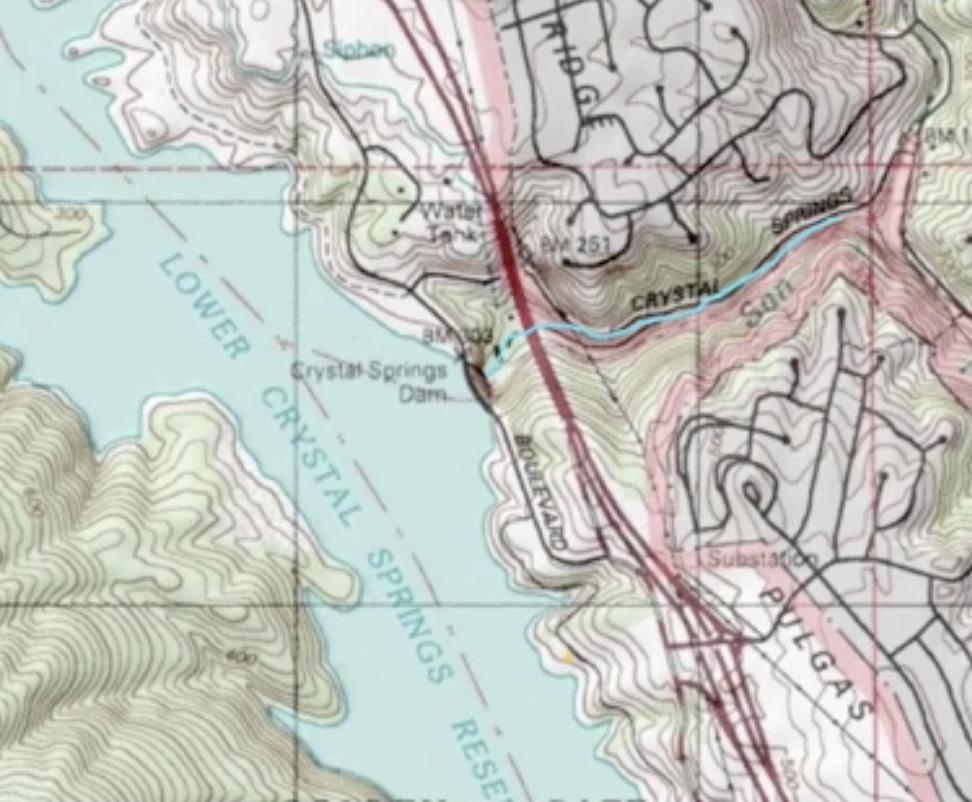
\includegraphics[width=.9\linewidth]{./Screen Shot 2020-09-02 at 8.37.26 PM.png}
\caption{Screen Shot 2020-09-02 at 8.37.26 PM.png}
\end{figure}

In a topological map, you could probably guess that the \textbf{steepest path
downwards/upwards is perpendicular to the lines.}

The constant voltage lines works in a similar way.

\subsection{Then, a Energy Thing.}
\label{sec:org378cc7e}
If we have an object in the air

Object

\_\{Air\}

..ground..

What is that object's gravitation potential energy?

\ldots{} \ldots{} \ldots{}

You will realize that I just asked a very dumb question. This is because
that \textbf{energy must be relative to something.} You must \emph{raise} the object
(giving us the \(\Delta h\) part of \(gpe = mg\Delta h\) to gain
gravitational potential energy.

\subsection{Electric Potential}
\label{sec:orgd64c844}
\definition{Electrical Potential}\{\(\frac{V}{C}\)\}
Voltage is a measure of how much electric potential energy (yes, it is
an \emph{energy} (in \(J\), joules)), would change per Couloub of energy that
is moved through.

Recall the energy example above. When you raise an object of \(1kg\)
from a place with elevation (\(\Delta h\)) \(10m\) to \(100m\), you
could represent the change in gravitation potential energy of that
operation as
\(mg \Delta h_1 - mg \Delta h_0 = m(g \Delta h_1-g \Delta h_0) = 1kg(9.8\frac{m}{s^2} 100m - 9.8\frac{m}{s^2} 10m)\).
Where, \(g\Delta h_1\) is a unit \(\frac{m^2}{s^2} = \frac{J}{kg}\).
Proving this last relationship is left as an excercise to the reader.

Funny way to write it, I know. But, we could take the equation
\(m(g \Delta h_1-g \Delta h_0)\) and use it as a perfect analogy for
using electric potential.

The amount of electric potential energy that would change by moving an
object of charge \(1C\) from a place with voltage (\(\Delta V\)) \(10V\)
to \(100V\), is \(Q_2(V_1-V_0) = 1C (100V-10V)\), where Voltage, \(V\),
represent the \emph{energy} potential --- analogous to, drumroll please,
\(\frac{J}{kg}\), except this time its \(\frac{J}{C}\).

\definition[Where $Q_2$ is the the charge in Coulombs $C$ of the test charge, and $V_1$ and $V_0$ are the electric potential values of the points the charge is being moved to and from]{Electric Potential Energy}{$Q_2(V_1-V_0)$}
\definition{Electric Potential, Volts}\{\(V = \frac{J}{C}\)\}
\end{document}
